\documentclass[final,12pt]{article}
\usepackage{graphicx}
\usepackage[letterpaper,margin=1.0in]{geometry}
\usepackage{amssymb}
\usepackage{changepage}
\usepackage{float}
\usepackage{hyperref}
\usepackage{url}
\usepackage{afterpage}
\usepackage{natbib}
\usepackage{setspace}
\usepackage{fancyhdr}
\usepackage{amsmath}
\usepackage{array}
\usepackage[table]{xcolor}
\pagestyle{fancy}
\fancyhf{}
\usepackage[latin1]{inputenc} 
\usepackage{lastpage}

\def\Student{OMAR ALEJANDRO ANGULO GIL}
\def\Title{}
\def\TitleESP{ANTEPROYECTO}
\def\Prog{Maestria en Ciencias (F\'{i}sica) }
\def\Dept{DIFUS}
\def\Institution{Universidad de Sonora}
\def\Director{Dr. Jos\'{e} Feliciano Ben\'{i}tez Rubio}
\def\ProjectTitle{Determination of the calibration constant for the 2025 luminosity measurement in the CMS experiment}
\def\ProjectTitleESP{}
\def\ResearchLine{F\'{i}sica de altas energ\'{i}as}

%%header and footer
\lhead{\Student}
\rhead{\TitleESP}
\rfoot{Page \thepage \hspace{1pt} of \pageref{LastPage}}

%%comands
\newcommand{\SubItem}[1]{ {\setlength\itemindent{15pt} \item[-] #1} }
\newcommand{\lumi}[1]{{#1~fb$^{-1}$}}
\newcommand{\instlumi}[1]{#1$\times 10^{34}$ cm$^{-2}$s$^{-1}$}
%\newcommand{\Lum}[1]{}

%%%%%%%%%%%%%%%%%%%%%%%%%%%%%%%%%%%%%
\begin{document}
\onehalfspacing

%%%%%%%%%%%%%%%%%%%%%%%%TITLE PAGE%%%%%%%%%%%%%%%%%%%%%%%%%%%5
\begin{titlepage}
\centering
\hspace{0pt}
%\vfill
{\scshape\Large \Title \\ \TitleESP \par}
%%project revised 2021-1
  
  \vspace{1cm}
  {
    TITLE:\par
    {\bf \large \ProjectTitle  \par}
       
    \vspace{0.4cm}
    %TITULO:\par
    %{\bf \large \ProjectTitleESP \par}
  }
       
  \vspace{1cm}
  {
    LGAC: \par
    \ResearchLine \par
  }
        
  \vspace{2cm}
  {\underline{\hspace{8cm}}\par}
  {\bf \scshape \Student \par}
  {Estudiante\par}

  \vspace{1cm}
  {\underline{\hspace{8cm}}\par}
  {\scshape \Director \par}
  {Director\par}

  \vspace{1cm}
  {\bf \Prog \par}
  %{\Dept \par}
  {\Institution \par}

  \vspace{2cm}
  {\today}

\hspace{0pt}
\vfill

\end{titlepage}


%%%%%%%%%%%%%%%%%%%%%%%%%%%% white page for print out %%%%%%%%%%%%%%%%%%%%%%%%%%%%%%%%%%%%
\shipout\null

%%%%%%%%%%%%%%55% Resumen %%%%%%%%%%%%%%%%%%%%%%%%%%%%%%%%%%%
\newpage
\begin{center}
  {\itshape\textbf{Resumen}\par}
\end{center}

\vspace{1 cm}

El proyecto busca realizar an�lisis y calibraci�n de los datos de luminosidad correspondiente a las mediciones hechas por el experimento CMS para la recta final de la Run 3, durante 2025. Se utiliza para la medici�n el m�todo PCC (por sus siglas en ingl�s, Pixel Cluster Counting) que consiste en el conteo de grupos de p�xeles activados en el detector. Esto nos permitir� medir con precisi�n el valor de luminosidad para los datos recabados durante este a�o. La luminosidad y su incertidumbre sistem�tica son par�metros de suma importancia para las mediciones de f�sica realizadas en los experimentos en el LHC.

\hspace{2pt}
\vfill

%%%%%%%%%%%%%%%%%%%%%%% Abstract Page %%%%%%%%%%%%%%%%%%%%%%%%%%%%%%
\newpage

  \begin{center}
    {\itshape\textbf{Abstract}\par}
  \end{center}
  
  \vspace{1 cm}
 
The projects seeks to analyze and calibrate the luminosity corresponding to the measurements made by the CMS experiment for the final stretch of run 3, during 2025. The method used to measure this is Pixel Cluster Counting (PCC), which consists in counting groups of activated pixels in the detector. This will let us measure with precision the value of the luminosity parameter for data collected this period. Along with its systematic uncertainty, luminosity are parameters of utmost importance for physics measurements in LHC experiments.   
   
  \hspace{2pt}
\vfill



%%%%%%%%%%%%%%%%%%%%%%%%%%%%%%%%%%%%%% Begin the body %%%%%%%%%%%%%%%%%%%%%%%%%%%%%
\newpage
\section{BACKGROUND}

The fundamental forces are the most elemental known interactions in nature, and the four recognized are gravity, electromagnetism, and the weak and strong forces. Gravity and electromagnestism are long-range interactions, and thus easily noticeable, while the weak and strong forces are essential to describe interatomic interactions. Particle physics, also refered as high energy physics, are in charge of studying said interactions, in addition to the fundamental particles that form all matter, and the standard model (SM) has been the most successful theoretical model, describing with precision these forces, with the important exception of gravity. The SM is separated between bosons, which are known as the mediators of the aforementioned forces, and fermions, consisting of elementary particles that compose every other particle.

In the fermionic sector, leptons and quarks fall into three generations: first generation has the up (u) and down (d) quarks, as well as the electron and electron neutrino; second generation consists of charm (c) and strange (s) quarks, muon and muon neutrino; and the third generation contains the top (t) and bottom (b), plus the tau and tau neutrino. Each one of these has its corresponding antiparticle, having their properties (such as charge) reversed in sign.  

On the other hand, the bosonic sector is composed of the gauge bosons, which mediate every interaction: the gluon ($g$) for the strong nuclear force, $W^{\pm}$ and $Z^0$ bosons for weak nuclear force, and the photon ($\gamma$) for electromagnetic force. The model also includes the Higgs boson ($H$), which is the way to account for the mass of other SM particles, via electroweak symmetry breaking mechanism \cite{Chatrchyan:2012xdj}.

Particles on the heavier side, such as the Higgs boson and the top quark (which were in fact, the last to be discovered), need a really high energy particle collider to be produced, like the Large Hadron Collider (LHC), that operates at a center-of-mass energy of 13.6 TeV in Geneva, Switzerland. It took multiple experiments, different colliders, and several years of upgrades on a long term plan to reach such high energies. So, it is indisputable that the energy of collision is one the most important parameter at particle colliders, but it is of similar significance to discuss and improve another parameter, called Luminosity.

Luminosity measures the number of useful events in a collider experiment. Instantaneous luminosity shows the ability of a particle accelerator to produce said interactions. It is the process-independent ratio between the rate of events per second $R(t)$, and the cross section of the process $\sigma_p$, and its defined by\\

\begin{equation}
  R=\mathcal{L}_{inst} \cdot \sigma_{p}\\
\end{equation}

To evaluate the total number of events, the integrated luminosity is used. It measures the collected data size, and characterizes the performance of an accelerator, given by:\\

\begin{equation}
  \mathcal{L}_{int} = \int _{0}^{t} \mathcal{L}(t') dt' \\ 
\end{equation}

During Run 1 (2011-2012) LHC reached a peak instantaneous luminosity of \instlumi{0.77} and delivered an integrated luminosity of about \lumi{25} with a precision of about 2.0\% 
\footnote{1 barn is a unit of area corresponding to $10^{-24}$ cm${^2}$ and 1 femtobarn (fb) = $10^{-39}$ cm$^{2}$. For comparison, the total Higgs production cross section is 48600 fb.}
In the first part of Run 2 (2015-2016), the delivered luminosity has been measured to be \lumi{38.4} with an unprecedented precision of 1.3\% \cite{Sirunyan:2021qkt}.
For the second part of Run 2 (2017-2018), the integrated luminosity is about \lumi{78}.
On the current LHC/HL-LHC plan, Run 3 began in 2022 and is planned to last until the first half of 2026, expecting and integrated luminosity of about \lumi{500}, as seen in figure \ref{figure1}.

\begin{figure}[H]
  \centering
  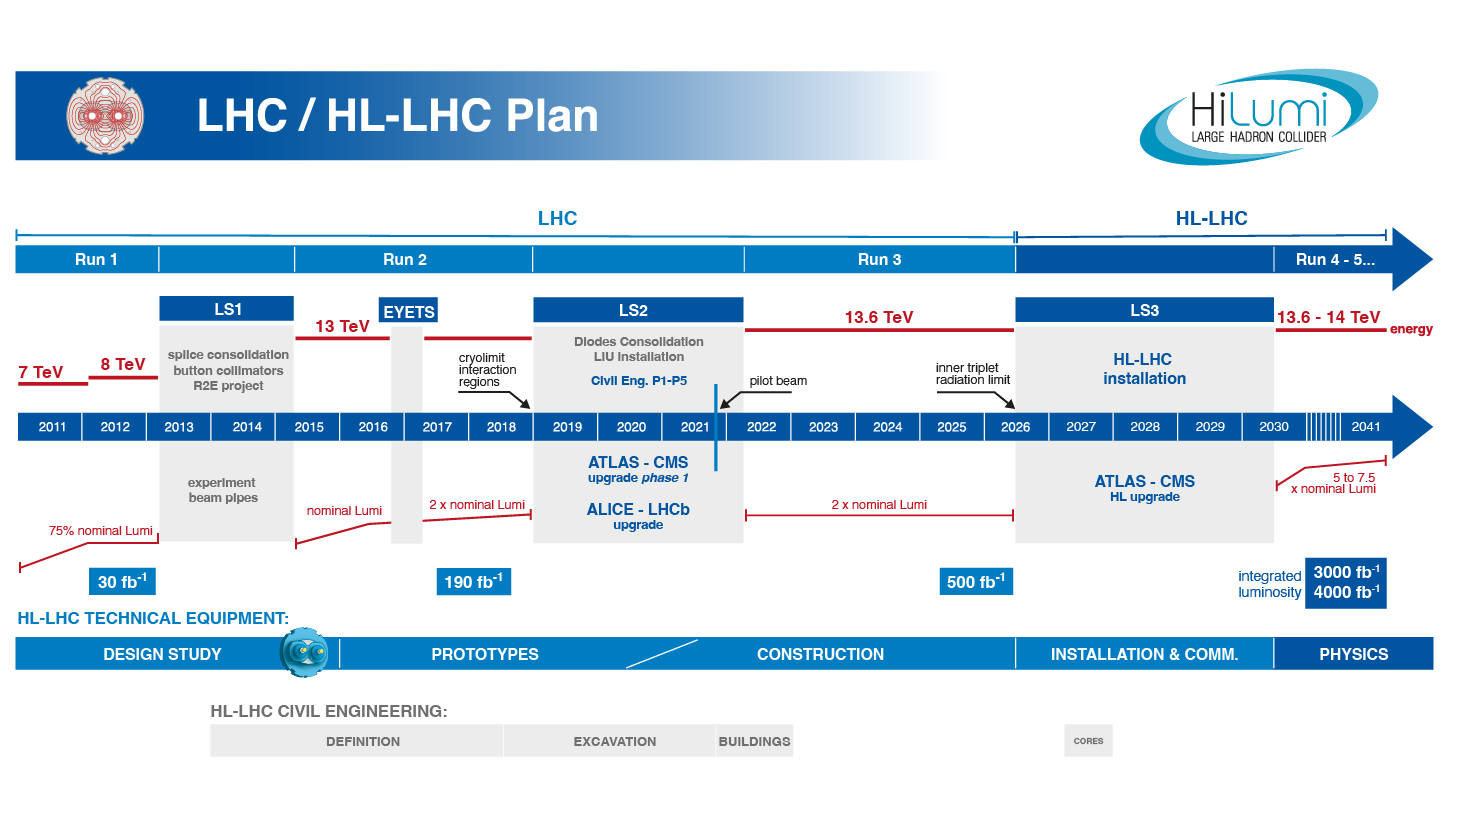
\includegraphics[width=0.85\columnwidth]{./LHCPlan.png}
  \caption{CERN's current plan for reaching the High Luminosity LHC. The Long Shutdown 3 (LS3) is now scheduled starting July 2026, seven and a half months later than planned, and with a duration increased by four months. The start of Run 4 is now programmed for 2030 \cite{Lamont_2024}.}
  \label{figure1}
\end{figure}

CERN's LHC has four major colliding points, each one with its respective detector: CMS, ATLAS, ALICE and LHCb. The detector that will be worked here corresponds to the CMS, which stands for Compact Muon Solenoid, and its experiment has the general objective to investigate a wide range of physics within the standard model and beyond, primarily with proton collisions.

The detector uses a powerful magnet to bend charged particles as they leave the point of collision, allowing to analyze its curvature to identify charge and measure their momentum. A silicon tracker, consisting of about 75 million sensors arranged in concentric layers, is in charge of measuring said curvature with high precision. It has the form of multiple cylindrical layers, and a large number of components. The electromagnetic calorimeter detects photons and electrons while the hadron calorimeter detects mostly pions ($\pi$) and kaons ($K$). Muons ($\mu$) are detected by special chambers outside the solenoid, as shown in \ref{figure3}. 

\begin{figure}[H]
  \centering
  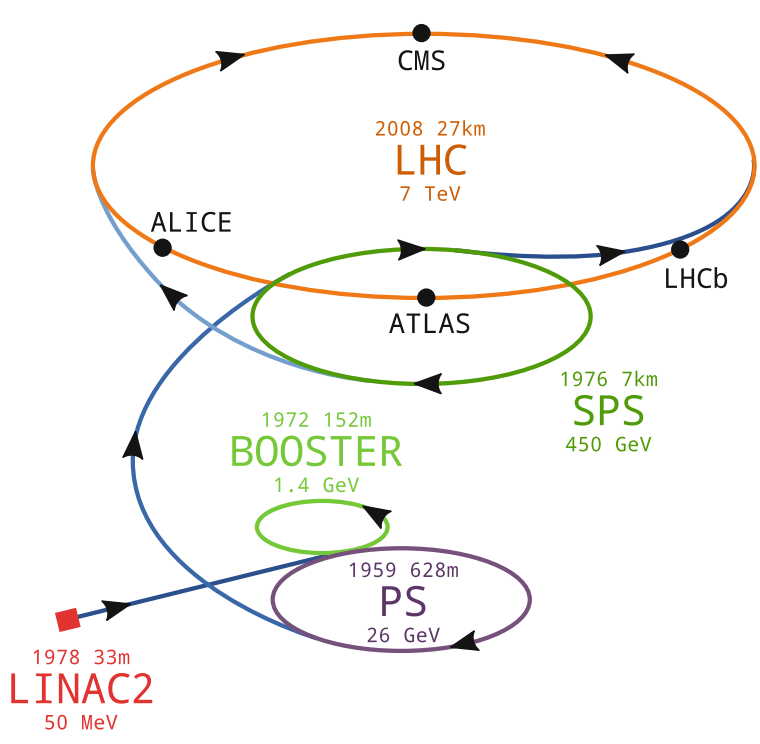
\includegraphics[width=0.6\columnwidth]{./LHCcomplex.png}
  \caption{Diagram of the LHC accelerator complex. It consists of three accelerator stages: the particle source, the Proton Synchrotron (PS), the Super Proton Synchrotron (SPS), and then the 27 km LHC ring. There are four collision points corresponding to the ALICE, ATLAS, LHCb, and CMS detectors  \cite{Mobs:2684277}.}
  \label{figure2}
\end{figure}

The CMS silicon pixel detector consists of four concentric cylindrical layers and three disks on each end, placed at certain distances from the center of the detector. The detector consists of 1856 sensor modules, and gives complete coverage over the interaction point, resulting in precise tracking. This yields a large amount of total pixels, so, adding the sensor's fine granularity, the hit occupancy is very low. Due to this, the Pixel Cluster Counting (PCC) method brings forth a linear function of pile up, which is an essential property of a luminometer. The PCC method has been used as one of main luminometers for more than a decade, showing its reliability.

\begin{figure}[H]
  \centering
  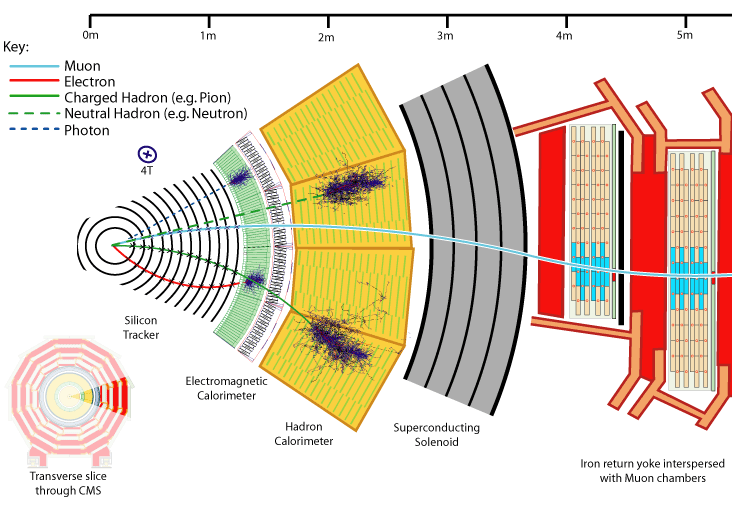
\includegraphics[width=0.7\columnwidth]{./cms12.png}
  \caption{Transverse cut of the CMS detector, showing the layers and disks mentioned, as well as the muon chambers \cite{Chatrchyan:2008aa}.}
  \label{figure3}
\end{figure}
  

%\begin{figure}[H]
  %\centering
  %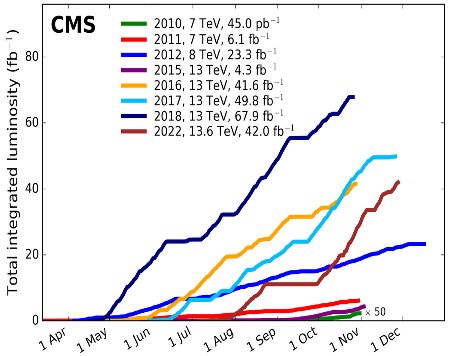
\includegraphics[width=0.45\columnwidth]{./integratedlum.png}
  %\caption{ }
  %\label{figure 3}
%\end{figure}
  
%%%%%%%%BUSCAR VERSION ACTUALIZADA DE ESTA%%%%%%%%%


\section{OBJECTIVE}

The objective is to analyze and calibrate the PCC luminometer for the 2025 recorded data by the CMS experiment, working with the PCC method and the van Der Meer (vdM) scans, allowing for a precise measurement of luminosity, and so, having access to more useful information to search for new discoveries.

\section{HYPOTHESIS}

Based on the analysis corresponding to previous years, a similar or better result is expected. With a systematic uncertainty of 1.4\% for 2022, and 1.3\% for 2023, it is possible to achieve a precision as good as this, if not an improvement.


\section{METHODOLOGY}

A pixel cluster is for a group of contiguous pixels activated by a charged particle. The method of choice, PCC, exploits the huge number of pixel in the interior part of the CMS pixel detector, which means that the probability that a single pixel is hit by two charged particles from the same bunch crossing is extremely small, so it yields measurements with a great linear response with the pile-up (number of interactions per bunch crossing, $\mu$). To calibrate the luminometer, the van der Meer (vdM) scan technique is employed in special runs, usually at the beginning of the year or period. The LHC has two main types of runs: physics runs (which could be proton-proton, heavy-ion, or proton-lead collisions) and callibration (or vdM) runs. As the title of the project suggests, callibration runs are the subject of study, and consist of more controlled collisions to be able to determine luminosity from the beam parameters.

% detector de pixeles

During the vdM runs, the pixel detector is recorded with a trigger of aproximately 50 kHz distributed 10 BCIDs of the 140 that collide, compared to the 2400 that colliding bunches on physics runs; and in turn, the pile-up is much less, giving $\mu \~ 0.5$, against an average of 57 in recent physics runs. The data is then distributed in 32 different datasets of events. %referencia pa la imagen de pile-up en runs de fisica

To ensure accurate and stable luminosity measurement, there is a detector module selection process, where a veto list is made each period and then combined for the entire year. This process involves determining the reliability of each module based on analyzing what is referred as the module weight, which is the change in the ratio of module PCC and total PCC. The veto list consists of modules excluded due to their long-term instabilities. At the end of said process, around 10\% of all modules are used. 

It is necessary to take into consideration a background noise contribution to the PCC rates. Each type of contribution is estimated independently during Super Separation (SS) periods, that are performed to separate two beams a certain distance for a selected period of time. To estimate the background value and its statistical error, the mean value and standard deviation are taken from the distribution resulting of the average of pixel clusters per event ($\langle PCC \rangle$).

% a couple graphs, maybe??

 The separation between proton beams is varied in two dimensions, in steps of 100 micrometers. It measures the rates of clusters using the PCC algorithm and the beam parameters during vdM, to determine the calibration constant ($\sigma_{vis}$). The instantaneous luminosity for a single colliding bunch pair can be calculated with the following formalism:

\begin{align}
  \mathcal{L}(\Delta x, \Delta y) &= N_1N_2f\int_{-\infty}^{\infty}\rho_1(x,y)\rho_2(x+\Delta x,y+\Delta y)dxdy \\
  &= N_1N_2f\int_{-\infty}^{\infty}\rho_1(x)\rho_2(x+\Delta x)dx\int_{-\infty}^{\infty}\rho_1(y)\rho_2(y+\Delta y)dy
\end{align}

Where $N_1$ and $N_2$ correspond to the number of protons in colliding bunches, $f = 11245.6$ Hz is the frequency of revolution of the LHC, and $\rho_i$ is the proton density distribution of the i-th bunch, assumed Gaussian. For the method to be applicable, it is assumed that the density distributions factorize in the tranverse direction $x$ and $y$, as shown above.

By integrating over either $\Delta$ (e.g. $x$)and substituting into (4), leads to

\begin{center}
  $\int\rho_1(y)\rho_2(y+\Delta y)dy=\frac{\int\mathcal{L}(\Delta x, \Delta y)d(\Delta x)}{N_1 N_2 f} \Rightarrow \mathcal{L}(\Delta x, \Delta y)=\int\rho_1(x)\rho_2(x+\Delta x)dx\int\mathcal{L}(\Delta x', \Delta y)d(\Delta x')$
\end{center}

and therefore

\begin{equation}
  \int\rho_1(x)\rho_2(x+\Delta x)dx=\frac{\mathcal{L}(\Delta x,\Delta y)}{\int\mathcal{L}(\Delta x', \Delta y)d(\Delta x')}
\end{equation}

Now, from equations (1), (4) and (5), taking $\Delta x=\Delta y=0$

\begin{equation}
  \mathcal{L}(0,0)=\frac{N_1N_2fR(0,0)R(0,0)}{\int R(\Delta x',0)d(\Delta x')\int R(0,\Delta y')d(\Delta y')}=\frac{N_1N_2f 2\pi}{\Sigma_x\Sigma_y}
\end{equation}

where the beam overlap widths $\Sigma_{x,y}$ are defined:

\begin{equation}
  \Sigma_{x,y}=\frac{1}{\sqrt{2\pi}}\frac{\int R_{x,y}(\Delta)d\Delta}{R_{x,y}(0)}
\end{equation}

and once again, from (1), we can define

\begin{equation}
  \sigma_{vis}=\frac{R(0,0)}{\mathcal{L}}=\frac{2\pi\Sigma_x\Sigma_yR(0,0)}{N_1N_2f}\\
\end{equation}
%%Si los dos haces son iguales, la dist estandar de ambas seria esta formula. El raiz de dos pi es asumiendo que las rho son distribuciones gaussianas

The parameter $\sigma_{vis}$ is known as the calibration constant, and is used to normalize the measured PCC rates so the luminosity can be determined during normal running throughout the data-taking year. In order to compute the constant, a mathematical function needs to be used to fit the averaged cluster rates, so the parameters needed, such as $\Sigma_{x,y}$ and $R(0,0)$, can be extracted. 

For the analysis, the quality of multiple functions is tested. The convergence of the function is the first evaluation on this quality, based on the covariance matrix and its status. Then, another important analysis is doing a $\chi^2$ test, which helps determine how likely a variable can come from a specified distribution. The value of $\chi^2$ is determined by

\begin{equation}
  \chi^2(\theta)=\sum_{i=1}^{N}\frac{(y_i-f(x_i,\theta))^2}{\sigma_i^2}
\end{equation}

where $y_i$ are the observed values measured with errors $\sigma_i$ at the values of $x_i$ given without error, with the theoretical value given by $f(x_i,\theta)$. How low the value of $\chi^2$ determines how good the fit is, and the parameter $\theta$ is adjusted to minimize it \cite{Statistical_Data_Analysis}.

After finishing the tests, the chosen fit model is used, and with corresponding noise corrections, the calibration constant can finally be calculated.

% Numero de colisiones entre protones (pileup) del total en un bonche (10^11)

\section{SPECIFIC OBJECTIVES}

To guarantee stable luminosity measurement for Run 3 2025, the set goals are:

\begin{itemize}
  \item Apply a selection of good modules from the detector: To assure an accurate measurement, a veto list is made, taking only modules with relatively consistent contributions, and then used to only process zero bias PCC data for the vdM analysis.
  \item Measure the noise in the modules: A calculation of the background contributions, made during selected time windows along every scan of the calibration program.
  \item Set the ideal model adjustment: The generated rates of the scan need to be fitted a mathematical function to extract the parameters needed. 
  \item Extract the beam parameters $\Sigma_i$, conducting scans in the $x$ and $y$ directions, determined through curved fitting of the scan data. 
  \item Compute the calibration constant $\sigma_{vis}$. 
  \item Determine the systematic uncertainties on the integrated luminosity: It is necessary to recognize the noise effects on the beam overlap measurement, and therefore the calculation of $\sigma_{vis}$, so corrections are to be applied.
\end{itemize}

\section{EXPECTED RESULTS}

The work done in this thesis project is expected to yield the following results:

\begin{itemize}
  \item Obtain the PCC luminometer calibration constant $\sigma_{vis}$ for the 2025 data.
  \item Estimate the background contribution for PCC during vdM calibration program.
  \item Calculate the systematic uncertainty.
\end{itemize}


\section{CALENDAR OF ACTIVITIES}

\begin{center}
  \begin{tabular}{|c|c|c|c|c|}
    \hline
    Task / Period & 2025-1 & Summer 2025 & 2025-2 & 2026-1 \\
    \hline
    Practice the programming tools & \cellcolor[HTML]{28B463} & \cellcolor[HTML]{28B463} & & \\
    \hline
    Study the literature involved & \cellcolor[HTML]{28B463} & \cellcolor[HTML]{28B463} & & \\
    \hline
    Estimate the background contribution & & & \cellcolor[HTML]{F4D03F} & \\
    \hline
    Test the fit functions & & & \cellcolor[HTML]{F4D03F} & \\
    \hline
    Calculate $\sigma_{vis}$ and its systematic uncertainty & & & \cellcolor[HTML]{F4D03F} & \\
    \hline
    Write the thesis & & & & \cellcolor[HTML]{E53935} \\
    \hline
    Present results at a congress & & & & \cellcolor[HTML]{E53935} \\
    \hline 
    Defend the thesis & & & & \cellcolor[HTML]{E53935} \\
    \hline
  \end{tabular}
\end{center}

\onehalfspacing
\bibliographystyle{unsrt} % y esto...........
\bibliography{paper}

\end{document}
